\documentclass [10pt,a4paper]{report}

\usepackage[utf8]{inputenc}
\usepackage{graphicx}
\begin{document}

\part{Le Grid5000}
	\chapter{Présentation du Grid5000}
Le Grid5000 est une grille informatique destinée à la recherche scientifique. Le projet a vu le jour en 2003 et a pour but de promouvoir la recherche sur les grilles informatiques en France. Le Grid5000 est aujourd'hui composé de 1200 noeuds répartis sur 9 sites différents situés en France et au Luxembourg et interconnectés avec le réseau Réseau National de télécommunications pour la Technologie l'Enseignement et la Recherche (RENATER). L'objectif du Grid5000 est de permettre aux scientifiques d'effectuer des expériences dans le domaine des systèmes informatiques et des réseaux distribués dans un environnement hétérogène aussi proche de la réalité que possible.

	\begin{figure}[!h]
		\centering
   		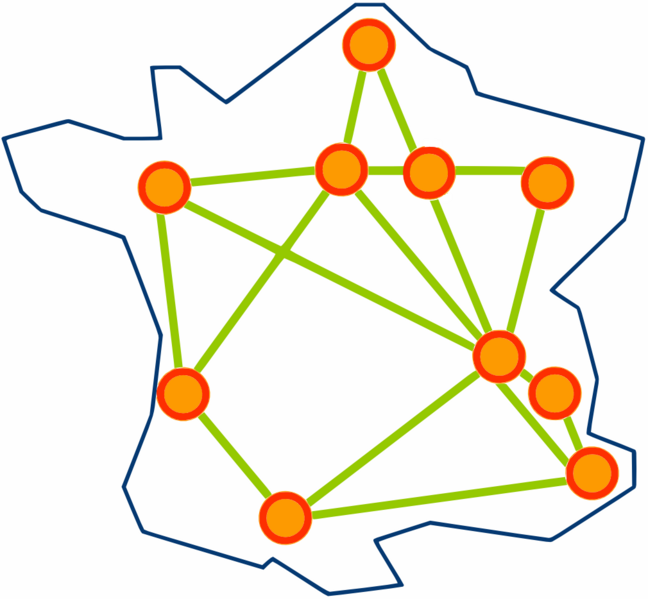
\includegraphics[width=5cm,height=5cm]{map.png}
   		\caption{Localisation des différents sites du Grid5000}
    	\label{fig:map}
	\end{figure} 

Le Grid5000 est donc composé de plusieurs sites distincts mais l'organisation au sein de chaque site est la même. Chaque site est composé d'un ou plusieurs clusters, c'est à dire un ensemble de machine homogène.Le site de Nancy par exemple héberge deux clusters nommés Griffon et Graphene. \\
A l'intérieur de chaque cluster se trouvent des ordinateurs aussi appelés "nodes" ou "noeuds". Il existe deux types de nodes : les noeuds de services et les noeuds de travail, sur lesquels sont efectuées les expériences. Les noeuds de services servent à l'administration des machines situées dans le cluster et à l'accès aux hôtes virtuels pour les administrateurs. Certains noeuds de services appelés "frontends" sont utilisés par les utilisateurs pour accéder aux différents sites grâce au protocole ssh, la réservation de noeuds et le déploiement. 

\begin{figure}[!h]
		\centering
   		\includegraphics[width=5cm,height=5cm]{griffon.jpeg}
   		\caption{Un des clusters de Nancy : Griffon}
    	\label{fig:griffon}
	\end{figure}
	
	\chapter{Les outils du Grid5000}
		Le Grid5000 est composé de plusieurs services: une partie ces services ont été développés uniquement pour ce projet comme par exemple Kadeploy3 qui a été developpé par l'INRIA Nancy - Grand Est; les autres sont des services standard déjà utilisés sur les systèmes Unix.  
		\section{OAR2}			
			OAR est un gestionnaire de ressources pour de grandes grilles informatique. Il est écrit en PERL et s'appuie sur une base SQL (PostgreSQL ou MySQL). OAR permet le déploiement, la réservation  et le management des noeuds et des jobs \footnote{un job correspond à une t\^ache affectée à une reservation}. OAR permet aussi d'effectuer des réservations planifiées de jobs pour une durée donnée en utilisant un nombre défini de noeuds. \\
			
		\section{Kadeploy3}
			Kadeploy est un outil qui permet le déploiement des différents systèmes d'exploitation sur les noeuds de la plateforme. Il permet aussi de configurer les noeuds, de les cloner et de les manager. Il permet le déploiement de système Linux, BSD, Windows et Solaris.
		\section{Taktuk}
			Taktuk est un outil complémentaire à OAR2. Taktuk permet l'éxecution de commandes à distance sur un grand nombre de noeuds hétérogènes. Il met en place un liaison entre la "frontends" et les noeuds concernées par la commande et s'adapte  à l'environnement de la machine (les perfomances , la charges , le réseau ...).  
		\section{KaVLAN}
			KaVLAN est un outil qui a pour but de permettre la mise en place d'un VLAN sur des noeuds du Grid5000. Il permet la mise en place de plusieurs type de VLAN : local, "router" et global. KaVLAN peut être utilisé en complément de Kadeploy et de OAR pour certains types d'expérimentation.\\
			\begin{itemize}
  				\item Un KaVLAN local est un VLAN complètement isolé du reste de la plateforme Grid5000. Il est alors obligatoire d'utiliser une gateway pour accéder aux noeuds se trouvant à l'intérieur de VLAN.
  				\item Un KaVLAN "router" permet l'accès à tous les noeuds du VLAN depuis le reste du Grid5000 sans utiliser de gateway.
 				 \item Un KaVLAN global est un VLAN qui est disponible sur tous les sites du Grid5000. Un routeur est alors configuré sur le site où le VLAN a été configuré.
			\end{itemize}
			
		\section{Les autres outils}
			Le Grid5000 utilise pour son fonctionnement d'autres outils :
				\begin{itemize}
					\item une base de donnée MySQL ou PostgreSQL. Cette base de donnée va \^etre utilisée par Kadeploy et OAR.
					\item un serveur DNS				
					\item un serveur DHCP
					\item un serveur NFS pour permettre aux utilisateurs de stocker des informations dans leur /home sur les différents sites.
				\end{itemize}
	
\end{document}
